\documentclass{article}
\title{Project 1}
\author{Nat Hawkins, Victor Ramirez, Mike Roosa, Pranjal Tiwari}
\date{26 Jan, 2017}

\usepackage{relsize,makeidx,color,setspace,amsmath,amsfonts,amssymb}
\usepackage[table]{xcolor}
\usepackage{bm,ltablex,microtype}
\usepackage{placeins}

\usepackage[top = 1in, bottom = 1in, right = 1in, left = 1in]{geometry}

\usepackage[pdftex]{graphicx}

\begin{document}
\maketitle

\begin{abstract}
The aim of this project is two-fold: primarily we aim to evaluate the limits of machine accuracy in the context of solving differential equations, and it functions as an introduction to problem solving in C++. We will be comparing the efficiency of vector and matrix methods of storage with respect to computation time while exercising basic C++ skills (i.e. dynamic memory allocation, compiling of cpp files, etc.). 
\end{abstract}
%The above is the abstract. Marked for return to add additional details.

\section{Introduction}
	Before we begin, although C++ will be used for some parts of this project in order to learn the language, the majority of our coding will be done in Python. The three of us have experience in using this language and we decided that it was best to play to our strengths in using the coding language we are most comfortable with. We will do some work with C++ and a discussion of this will be provided in our report. 
	
	\subsection{Mathematical Motivation}
		The motivation behind this project is simple: Many important differential equations in  Science can be written as 	linear second-order differential equations
		\begin{equation*}
		\frac{d^2y}{dx^2}+k^2(x)y = f(x),
		\end{equation*}
		where $f$ is normally called the inhomogeneous term and $k^2$ is a real function.
		
		A classical equation from electromagnetism is Poisson's equation.	The electrostatic potential $\Phi$ is generated by a localized charge distribution $\rho (\mathbf{r})$.   In three dimensions it reads
		
		\begin{equation*}
		\nabla^2 \Phi = -4\pi \rho (\mathbf{r}).
		\end{equation*}
		With a spherically symmetric $\Phi$ and $\rho (\mathbf{r})$  the equations
		simplifies to a one-dimensional equation in $r$, namely
		
		\begin{equation*}
		\frac{1}{r^2}\frac{d}{dr}\left(r^2\frac{d\Phi}{dr}\right) = -4\pi \rho(r),
		\end{equation*}
		which can be rewritten via a substitution $\Phi(r)= \phi(r)/r$ as
		
		\begin{equation*}
		\frac{d^2\phi}{dr^2}= -4\pi r\rho(r).
		\end{equation*}
		The inhomogeneous term $f$ or source term is given by the charge distribution
		$\rho$  multiplied by $r$ and the constant $-4\pi$.
		
		We will rewrite this equation by letting $\phi\rightarrow u$ and 
		$r\rightarrow x$. 
		The general one-dimensional Poisson equation reads then
		
		\begin{equation*}
		-u''(x) = f(x).
		\end{equation*}
		

\section{Solution}
\subsection{Problem Set-Up}
In this project we solved the one-dimensional Poisson equation with Dirichlet boundary conditions by rewriting it as a set of linear equations.

In doing so, our mathematics looked something like the following:

\begin{equation*}
-u''(x) = f(x), \hspace{0.5cm} x\in(0,1), \hspace{0.5cm} u(0) = u(1) = 0.
\end{equation*}

In our case we will assume  that the source term is 
$f(x) = 100e^{-10x}$, and keep the same interval and boundary  conditions. Then the above differential equation
has a closed-form  solution given by \\$u(x) = 1-(1-e^{-10})x-e^{-10x}$. We will compare
our numerical solution with this result in the future exercise.

We fed the program an input value $i$, which was then used to determine $x$ and the step size $h$. We did this by defining the variables as follows
\begin{equation*}
i = [input], \hspace{0.5cm} n = 10^{i},\hspace{0.5cm}  h = \frac{1.0}{n}
\end{equation*}

We  approximate the second derivative of $u$ with
\begin{equation*}
-\frac{v_{i+1}+v_{i-1}-2v_i}{h^2} = f_i  \hspace{0.5cm} \mathrm{for} \hspace{0.1cm} i=1,\dots, n,
\end{equation*}
where $f_i=f(x_i)$.



We began with a tridiagonal matrix, A, and transformed the problem into the following:

\begin{equation*}
\mathbf{A}\mathbf{v} = \tilde{\mathbf{b}},
\end{equation*}
where $\mathbf{A}$ is an $n\times n$  tridiagonal matrix which we rewrite as

\[
\mathbf{A} = \begin{bmatrix}
2& -1& 0 &\dots   & \dots &0 \\
-1 & 2 & -1 &0 &\dots &\dots \\
0&-1 &2 & -1 & 0 & \dots \\
& \dots   & \dots &\dots   &\dots & \dots \\
0&\dots   &  &-1 &2& -1 \\
0&\dots    &  & 0  &-1 & 2 \\
\end{bmatrix},
\]
and $\tilde{b}_i=h^2f_i$.  A can be derived by looking at the formula for the approximation of the second derivative. Note how the $v_{i+1}$ and the $v_{i-1}$ terms have a coefficient of $-1$. This is where the off diagonal elements come from in our matrix A. Since the two off diagonal entries are equivalent, we can approximate them into one vector, $e$. However, since all of the entries are -1, we decided to not allocate memory to this. Instead, we simplified our algorithm to account for these values. We will discuss our problem solving algorithms in the following section.

The reason for the conversion from a matrix to vectors comes about in our number of floating point operations (FLOPS). In using the matrix approximation, we were looking at (reference) $~\frac{2}{3}n^{3}$ FLOPS in calculating our solutions. However, in being able to reduce this down to a vector problem, we managed to reduced our calculations to $9n$, and then further to $4n$, again to be discussed in the next section. The short of this discussion is that we were able to reduce our floating point operations by two orders of magnitude. In the sense of computational efficiency, this makes for much smarter problem solving and much more effective computation. 

\subsection{Algorithms}
The algorithms that we implemented in the solving of this problem are as follows. We denote the dioagonal elements as $d[i]$, the solution values as $u[i]$, and the values of the function as $f[i]$. The problem starts when look at a general case for a $4$x$4$ matrix:

\[
\mathbf{A} = \begin{bmatrix}
d_{1}& e_{1}& 0& 0& \\
e_{1}& d_{2}& e_{2}& 0& \\
0& e_{2}& d_{3}& e_{3}& \\
0& 0& e_{3}& d_{4}& \\
\end{bmatrix},
\
\
\mathbf{u} = \begin{bmatrix}
u_{1}\\
u_{2} \\
u_{3}\\
u_{4}\\
\end{bmatrix},
\
\
\mathbf{f} = \begin{bmatrix}
f_{1}\\
f_{2} \\
f_{3}\\
f_{4}\\
\end{bmatrix},
\]

And now we can look at solving $\mathbf{A}\mathbf{u} = \tilde{\mathbf{f}},$ through the process of Gaussian Elimination. For this process, reference (reference). In essence, we begin by multiplying the second row of $A$ by the ratio of the terms in the first column of rows one and two. Explicitly, this looks like $\frac{e_{1}}{d_{1}}$ on both the right hand side and left hand side. This transforms the equation into the following: 

\[
\begin{bmatrix}
d_{1}& e_{1}& 0& 0& \\
0& d_{2}-\frac{e_{1}^{2}}{d_{1}}& e_{2}& 0& \\
0& e_{2}& d_{3}& e_{3}& \\
0& 0& e_{3}& d_{4}& \\
\end{bmatrix}
*
\begin{bmatrix}
u_{1}\\
u_{2} \\
u_{3}\\
u_{4}\\
\end{bmatrix}
=
\begin{bmatrix}
f_{1}\\
f_{2} - f_{1} \frac{e_{1}}{d_{1}} \\
f_{3}\\
f_{4}\\
\end{bmatrix}
\]

We now can redefine $\tilde{d_{2}}= d_{2}-\frac{e_{1}^{2}}{d_{1}}$ and $\tilde{f_{2}} = f_{2} - f_{1} \frac{e_{1}}{d_{1}} $. This changes the matrix to a new form that we can use to repeat the process further.

\[
\begin{bmatrix}
d_{1}& e_{1}& 0& 0& \\
0& \tilde{d_{2}}& e_{2}& 0& \\
0& e_{2}& d_{3}& e_{3}& \\
0& 0& e_{3}& d_{4}& \\
\end{bmatrix}
*
\begin{bmatrix}
u_{1}\\
u_{2} \\
u_{3}\\
u_{4}\\
\end{bmatrix}
=
\begin{bmatrix}
f_{1}\\
\tilde{f_{2}}\\
f_{3}\\
f_{4}\\
\end{bmatrix}
\]

Now, we can perform the same operation and multiply the second row by $\frac{e_{2}}{\tilde{d_{2}}}$. As we now with Gaussian Elimination, the final result will be an upper triangular matrix of the form:

\[
\begin{bmatrix}
	d_{1}& e_{1}& 0& 0& \\
	0& \tilde{d_{2}}& e_{2}& 0& \\
	0& 0& \tilde{d_{3}}& e_{3}& \\
	0& 0& 0& \tilde{d_{4}}& \\
\end{bmatrix}
*
\begin{bmatrix}
	u_{1}\\
	u_{2} \\
	u_{3}\\
	u_{4}\\
\end{bmatrix}
=
\begin{bmatrix}
	f_{1}\\
	\tilde{f_{2}}\\
	\tilde{f_{3}}\\
	\tilde{f_{4}}\\
\end{bmatrix}
\]

At this point, we can begin the process of forward substitution and equate $\tilde{d_{4}} * u_{4} = \tilde{f}_{4}$. Using this value, we can solve for $u_{4}$ and then solve $\tilde{d_{3}} * u_{3} + \tilde{d_{4}} * u_{4} = \tilde{f}_{3}$ for $u_{3}$, and so on and so forth. With pre-populated arrays for $u$ and $f$, we now have our solution. We can now extend this process to a more general case for a square matrix of any size. This process yields the algorithms used in our program.


\begin{align}
\tilde{d_{i}} &= d_{i}-\frac{e_{i-1}^{2}}{d_{i-1}} \\
\tilde{f_{i}} &= f_{i} - f_{i-1} \frac{e_{i-1}}{d_{i-1}} \\
u_{i} &= \frac{	\tilde{f}_{i} - e_{i}u_{i+1}}{d_{3}}
\end{align}

Now we can use the fact that for our specific case all of the $e_{i}$ values are equal to -1 to simplify our algorithms. This also causes a drastic simplification for the $d_{i}$ values. 

\begin{align}
\tilde{d_{i}} &= \frac{i+1}{i} \\
\tilde{f_{i}} &= f_{i} + f_{i-1} \frac{1}{d_{i-1}} \\
u_{i} &= \frac{	\tilde{f}_{i} + u_{i+1}}{d_{3}}
\end{align}

Thus, we see a reduced floating point operation count down to $\approx 4n$. This is where the efficiency of this approach really becomes evident. 

Some examples of our code can be seen in \textbf{Figure 1}.
\begin{figure}[h!]
	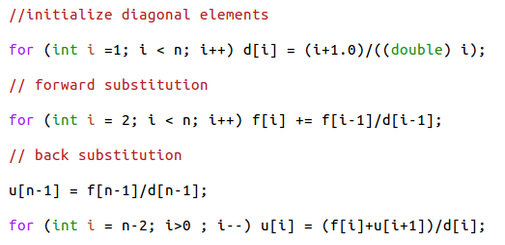
\includegraphics[width=\linewidth]{codesample.png}
	\caption{The figure above shows the iterative loops that we used in C++ to initialize these quantities and calculate further ones. Note the simplified algorithms were used in our code to reduce floating point operations.}
	\label{fig:codesample}
\end{figure}

\subsection{Problem 1c}

\subsection{Relative Error}
We calculated the relative error in the data set $i=1,\dots, n$,by setting up

\[
\epsilon_i=log_{10}\left(\left|\frac{v_i-u_i}
{u_i}\right|\right),
\]
as function of $log_{10}(h)$ for the function values $u_i$ and $v_i$. Here, it is important to note that the i value corresponds to the step size, $h$, as discussed above as $h = \frac{1.0}{n}$. The relative error was calculated for each power of ten, corresponding to an input value, $i$.
For each step length, we saw that the error was pretty much a constant, meaning that for each value of $x$, the relative error was approximately the same. Since the error was the exact same for all x values, we elected to sample only one error entry \textbf{ specifically the first entry} for the sake of efficiency (i.e. $i=1, x= 0.1 \hspace{0.5cm} i=2, x = 0.01, etc.$). This is a standard practice for looking at error trends. We were consistent with our choice, so whatever error that this may have imposed, we were at least consistent with this and can account it to systematic error. We then conducted multiple trials utilizing values of $i$ ranging from $i=0$ to $i=8$. Or, step sizes ranging from $10^{-6} \rightarrow 10^{-8}$. The results we got are plotted in \textbf{Figure 2}.

\begin{figure}[h!]
	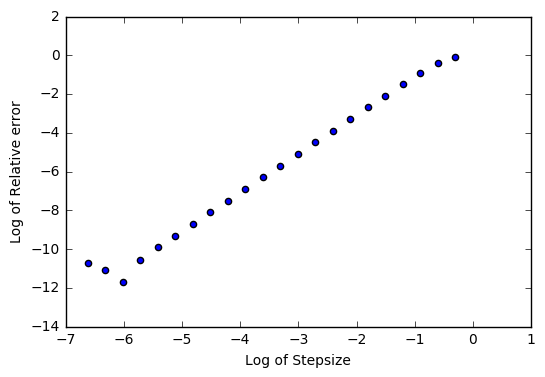
\includegraphics[width=\linewidth]{PHY480_P1_RerrvSs.png}
	\caption{Plot of Log of Relative Error. On the x-axis, we see the log of the step-size. This is equivalent to looking at which $i$ value we chose to use in order to approximate our solution. The y-axis shows the log of the relative error given in the equation above. What we see is that the log of error has a slope of approximately -2, as expected in our initial mathematic discussion. The error begins to increase again after $i=6$ or $n=10^{6}, h \approx 10^{-6}$. This is due to the truncation error that is getting overwritten by the number of bits. The increase in error can be accounted to machine error.}
	\label{fig:errorplot}
\end{figure}

\newpage
\subsection{LU Decomposition Comparison}
We then, as part of our work, wanted to work through this problem but utilizing LU decomposition. The process of LU decomposition is describe in the process in our algorithms section. For further discussion on this topic, see (reference to textbook that describes this process). 

The code that we used to set up the LU decomposition is described in \textbf{Figure 3}.

\begin{figure}[h!]
	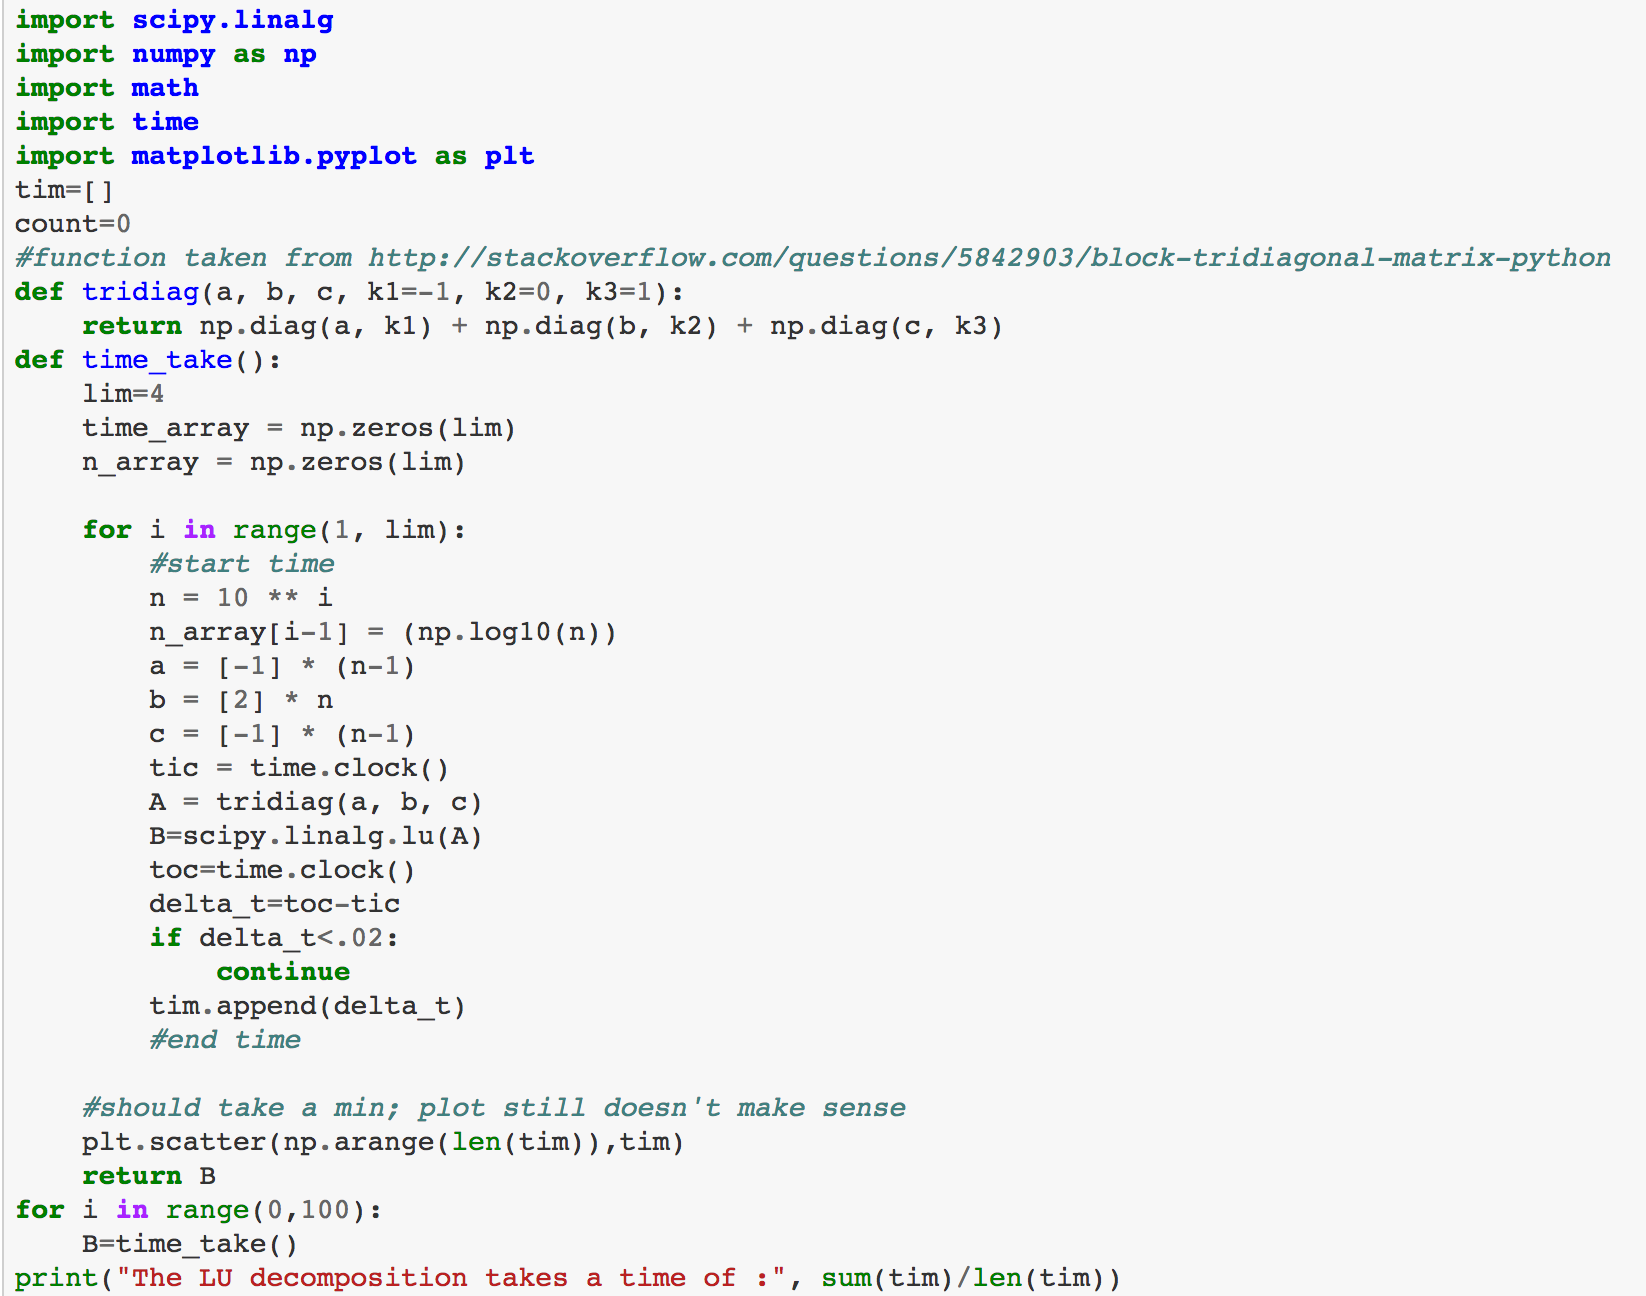
\includegraphics[width = \linewidth]{LUcode.png}
	\caption{Our Sample code in Python that details the process of setting up our matrices and then performing the LU decomposition. This process also tracks the time needed to complete the program.}
	\label{fig:LUcode}
\end{figure}

To make this matrix, we actually took some code from online to initialize the tridiagonal matrix. The code was obtained from (reference). Basically, what the code does is it doesn't make a matrix, as a nxn matrix would take a massive amount of memory, so it creates 3 arrays, which correspond to the 3 diagonals that have non-zero numbers within the tridiagonal matrix. Much of the code is actually to create the matrix, and there is a module in numpy which actually does the LU-decomposition, so we didn't have to hard code the process in. But to see how long this process takes, we used the time.clock function from the time module and took the difference in times between the end of initializing the matrix and completing the LU-decomposition process. Then we ran the code 100 times and made a scatter plot of the time this took. We took the average time and found that to make a 1000x1000 matrix, it took an average of about .06 s to complete the code.

\begin{figure}
	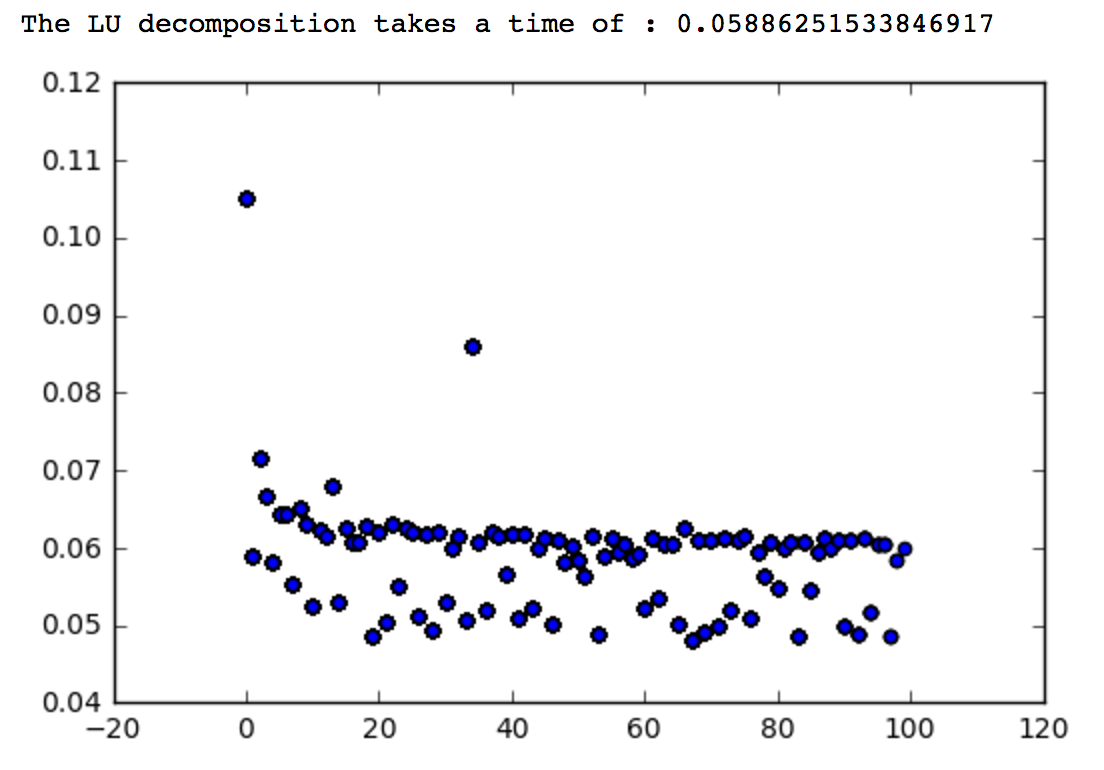
\includegraphics[width = \linewidth]{timeplot.png}
	\caption{The plot above shows the trials for LU decomposition that we ran to calculate the time that it takes to achieve our numerical results. The x-axis denotes the trial number (just an integer associated with trial 1,2,3,... etc.) and the y-axis was the time that the program took to complete in seconds. The final result was an average time over 100 trials.}
\end{figure}

The LU decomposition of the matrix was then used to solve for the solution to the differential equation as we did using our algorithms in our earlier code. While this may seem like an incredibly fast process, but the true difference became noticeable when we looked at larger matrices. For the $10^{4}$x$10^{4}$ and $10^{5}$x$10^{5}$ cases, the amount of memory required ot complete the calculations and the time necessary to compile the code caused errors in our computer systems. Thus, we saw the fatal error of this approach. For our general case using simplified algorithms, we were able to effectively solve the differential equations for matrices up to the order of $10^{8}$x$10^{8}$ case without issue. The amount of time and memory required to use LU decomposition for the sake of solving differential equations of this form make this an ineffective method. 

Also, fun fact, it takes 42 minutes, roughly, to compile the $10^{5}$ square matrix case.

\newpage
\section{Conclusions}


\section{References}
\begin{enumerate}
	\item  Block tridiagonal matrix python. (n.d.). Retrieved January 27, 2017, from http://stackoverflow.com/questions\\/5842903/block-tridiagonal-matrix-python
	
	\item https://github.com/CompPhysics/ComputationalPhysicsMSU , This is a github repository, which had some code in it that we used in our ipython notebooks.
	
	\item Press, W. H., Vetterling, W. T., Teukolsky, S. A., and Flannery, B. P. (1992). \textit{Numerical recipes in C. the art of scientific computing}. Cambridge University Press.
\end{enumerate}



\end{document}